% This file was created (at least in part) by the script ParseMdtoLatex by Louis du Plessis
% (Available from https://github.com/taming-the-beast)

\documentclass[11pt]{article}
%%%%%%%%%%%%%%%%%%%%%%%%%%%%%%%%%%%%%%%%%%%%%%%%%%%%%%%%%%%%%%%
% DO NOT EDIT THIS FILE UNLESS YOU KNOW WHAT YOU ARE DOING!!! %
%%%%%%%%%%%%%%%%%%%%%%%%%%%%%%%%%%%%%%%%%%%%%%%%%%%%%%%%%%%%%%%

\usepackage[]{authblk}
\usepackage{graphicx}
\usepackage{color}
\usepackage{longtable}
\usepackage{hanging}
\usepackage{indentfirst}
\usepackage{setspace}
\usepackage{enumitem}
\usepackage{verbatim}
\usepackage{upgreek}
\usepackage{framed}
\usepackage{textcomp}
\usepackage{url}
\usepackage{soul}
\usepackage{amsmath, amsfonts,amssymb,mathrsfs}
\usepackage{fancyhdr}
\usepackage[compact]{titlesec}
\usepackage[T1]{fontenc}
\usepackage{lmodern}

\usepackage[backend=bibtex,hyperref=true,citestyle=authoryear,bibstyle=authortitle,firstinits=true,terseinits=true,doi=false,url=false,eprint=false,maxbibnames=10,maxcitenames=2]{biblatex}
\DeclareCiteCommand{\cite}
  {\usebibmacro{prenote}}
  {\usebibmacro{citeindex}%
   \printtext[bibhyperref]{\usebibmacro{cite}}}
  {\multicitedelim}
  {\usebibmacro{postnote}}

\DeclareCiteCommand*{\cite}
  {\usebibmacro{prenote}}
  {\usebibmacro{citeindex}%
   \printtext[bibhyperref]{\usebibmacro{citeyear}}}
  {\multicitedelim}
  {\usebibmacro{postnote}}

\DeclareCiteCommand{\parencite}[\mkbibparens]
  {\usebibmacro{prenote}}
  {\usebibmacro{citeindex}%
    \printtext[bibhyperref]{\usebibmacro{cite}}}
  {\multicitedelim}
  {\usebibmacro{postnote}}

\DeclareCiteCommand*{\parencite}[\mkbibparens]
  {\usebibmacro{prenote}}
  {\usebibmacro{citeindex}%
    \printtext[bibhyperref]{\usebibmacro{citeyear}}}
  {\multicitedelim}
  {\usebibmacro{postnote}}

\DeclareCiteCommand{\footcite}[\mkbibfootnote]
  {\usebibmacro{prenote}}
  {\usebibmacro{citeindex}%
  \printtext[bibhyperref]{ \usebibmacro{cite}}}
  {\multicitedelim}
  {\usebibmacro{postnote}}

\DeclareCiteCommand{\footcitetext}[\mkbibfootnotetext]
  {\usebibmacro{prenote}}
  {\usebibmacro{citeindex}%
   \printtext[bibhyperref]{\usebibmacro{cite}}}
  {\multicitedelim}
  {\usebibmacro{postnote}}

\DeclareCiteCommand{\textcite}
  {\boolfalse{cbx:parens}}
  {\usebibmacro{citeindex}%
   \printtext[bibhyperref]{\usebibmacro{textcite}}}
  {\ifbool{cbx:parens}
     {\bibcloseparen\global\boolfalse{cbx:parens}}
     {}%
   \multicitedelim}
  {\usebibmacro{textcite:postnote}}

\newcommand{\citep}{\parencite}
\newcommand{\citet}{\textcite}
\defbibheading{relevref}[\refname]{\section*{Relevant References}}

\renewcommand{\postnotedelim}{\iffieldpages{postnote}{\addcolon}{\addcomma\space}} 
\DeclareFieldFormat{postnote}{#1} 

\DeclareFieldFormat[article, inbook, incollection, inproceedings, patent, thesis, unpublished]{title}{#1}
\DeclareFieldFormat[article, inbook, incollection, inproceedings, patent, thesis, unpublished]{journaltitle}{\mkbibemph{#1}\nopunct}
\DeclareFieldFormat[article, inbook, incollection, inproceedings, patent, thesis, unpublished]{volume}{{#1}\addcolon} %puts volume number in parens
%\DeclareFieldFormat[article, inbook, incollection, inproceedings, patent, thesis, unpublished]{year}{\mkbibparens{#1}\nopunct} %puts year in parens

\DeclareFieldFormat[article, incollection, patent, thesis, unpublished]{pages}{{\nopp#1}}

\DeclareFieldFormat{sentencecase}{\MakeSentenceCase{#1}}

\renewbibmacro*{title}{%
  \ifthenelse{\iffieldundef{title}\AND\iffieldundef{subtitle}}
    {}
    {\ifthenelse{\ifentrytype{article}\OR\ifentrytype{inbook}%
      \OR\ifentrytype{incollection}\OR\ifentrytype{inproceedings}%
      \OR\ifentrytype{inreference}}
      {\printtext[title]{%
        \printfield[sentencecase]{title}%
        \setunit{\subtitlepunct}%
        \printfield[sentencecase]{subtitle}}}%
      {\printtext[title]{%
        \printfield[titlecase]{title}%
        \setunit{\subtitlepunct}%
        \printfield[titlecase]{subtitle}}}%
     \newunit}%
  \printfield{titleaddon}}

\DefineBibliographyStrings{english}{% various adjustments to common bib entry strings
urlseen = {Accessed:},% What goes in front of the date a URL was accessed/retrieved etc.
editor = {(Ed)},%Ed – no dot, in brackets
editors = {(Eds)},% Eds – no dot, in brackets
byeditor = {(Ed.)}}% ‘Edited by’ for edited works

\DeclareNameAlias{default}{last-first}

\renewbibmacro{in:}{}

\renewbibmacro{publisher+location+date}{
  \iflistundef{publisher}
    {}
    {\printlist{publisher}%
       {\addcomma\space}%
      \iflistundef{location}
        {}
        {\printlist{location}}%
    }
}

\DeclareBibliographyDriver{article}{%
\usebibmacro{bibindex}%
\usebibmacro{begentry}%
\usebibmacro{author/translator+others}%
\newunit\newblock
\printfield{year}%
\setunit{\labelnamepunct}\newblock
\usebibmacro{title}%
\newunit
\printlist{language}%
\newunit\newblock
\usebibmacro{byauthor}%
\newunit\newblock
\usebibmacro{bytranslator+others}%
\newunit\newblock
\printfield{version}%
\newunit\newblock
%\usebibmacro{in:}% %mit in:
\usebibmacro{journal}%
\newunit\newblock
\printfield{volume}%
\newunit\newblock
\usebibmacro{byeditor+others}%
\newunit\newblock
\usebibmacro{note+pages}%
\newunit\newblock
\iftoggle{bbx:isbn}
{}%
\newunit\newblock
\usebibmacro{doi+eprint+url}%
\newunit\newblock
\usebibmacro{addendum+pubstate}%
\newunit\newblock
\usebibmacro{pageref}%
\usebibmacro{finentry}}

\DeclareBibliographyDriver{inproceedings}{%
\usebibmacro{bibindex}%
\usebibmacro{begentry}%
\usebibmacro{author/translator+others}%
\newunit\newblock
\printfield{year}%
\setunit{\labelnamepunct}\newblock
\usebibmacro{title}%
\newunit
\printlist{language}%
\newunit\newblock
\usebibmacro{byauthor}%
\newunit\newblock
\usebibmacro{bytranslator+others}%
\newunit\newblock
\printfield{version}%
\newunit\newblock
%\usebibmacro{in:}% %mit in:
\usebibmacro{booktitle}%
\newunit\newblock
\printfield{volume}%
\newunit\newblock
\usebibmacro{byeditor+others}%
\newunit\newblock
\usebibmacro{publisher+location+date}%
\newunit\newblock
\usebibmacro{note+pages}%
\newunit\newblock
\usebibmacro{pageref}%
\usebibmacro{finentry}}

\DeclareBibliographyDriver{book}{%
\usebibmacro{bibindex}%
\usebibmacro{begentry}%
\usebibmacro{author/translator+others}%
\newunit\newblock
\printfield{year}%
\setunit{\labelnamepunct}\newblock
\usebibmacro{title}%
\newunit
\printlist{language}%
\newunit\newblock
\usebibmacro{byauthor}%
\newunit\newblock
\usebibmacro{bytranslator+others}%
\newunit\newblock
%\usebibmacro{in:}% %mit in:
\usebibmacro{booktitle}%
\newunit\newblock
\printfield{volume}%
\newunit\newblock
\usebibmacro{publisher+location+date}%
\newunit\newblock
\usebibmacro{note+pages}%
\newunit\newblock
\usebibmacro{pageref}%
\usebibmacro{finentry}}




\setlist{nolistsep}

\setlength{\evensidemargin}{0in}
\setlength{\headheight}{0in}
\setlength{\headsep}{0in}
\setlength{\oddsidemargin}{-0.25in}
\setlength{\paperheight}{11in}
\setlength{\paperwidth}{8.5in}
\setlength{\tabcolsep}{0in}
\setlength{\textheight}{9in}
\setlength{\textwidth}{7in}
\setlength{\topmargin}{0in}
\setlength{\topskip}{0in}
\setlength{\voffset}{0in}
\parskip = 0.15in
\pagestyle{plain}
\setlength{\parindent}{0cm}

\definecolor{citescol}{RGB}{194,101,1}
\definecolor{urlscol}{RGB}{0,150,206}
\definecolor{linkscol}{RGB}{149,0,207}
\definecolor{mycol}{RGB}{25,23,191}
\definecolor{outputcol}{RGB}{34,139,34}
\definecolor{tcol}{RGB}{165,0,14}


\DeclareMathAlphabet{\msfsl}{T1}{cmr}{m}{it}
\DeclareMathAlphabet{\msyf}{OMX}{pcr}{m}{it}
\newcommand{\alf}{\upalpha}
\newcommand{\hilight}[1]{\colorbox{yellow}{#1}}

\newcommand{\levelone}[1]{
\bigskip
\noindent{\LARGE{\textsc{#1}}}
\vspace {0.05in}
}

\newcommand{\leveltwo}[1]{
\bigskip
\noindent{\Large{\textit{#1}}}
\vspace {-1mm}
}

\newcommand{\descriptionhead}[1]{
\noindent{\textcolor{mycol}{\textbf{\textit{#1}}}}\\ \vspace{-7mm}
}

\newcommand{\dhead}[1]{
\noindent{\textbf{\textit{#1 --}}}
}



\newcommand{\exs}[1]{
\vspace{-4mm}
\begin{itemize}
\item #1 \\ \vspace{-8mm}
\end{itemize}
}

\newcommand{\nbo}[1]{{\color{red}{#1}}}


\newcommand{\stepbullet}{\noindent \textbullet \ }
\newcommand{\mi}[1]{\textbf{\textit{#1}}}


\newcommand{\levelthree}[1]{\textit{#1 --}}


%\bibliographystyle{apalike}
%\bibpunct[; ]{(}{)}{;}{a}{,}{;}


\usepackage[breaklinks]{hyperref}
\usepackage[all]{hypcap}
\hypersetup{colorlinks=true,linkcolor=linkscol,citecolor=citescol,urlcolor=urlscol}


\newcommand{\R}{\texttt{R} }
\newcommand{\TESS}{\texttt{TESS}}
\newcommand{\PBD}{\texttt{PBD}}
\newcommand{\DDD}{\texttt{DDD}}
\newcommand{\Laser}{\texttt{laser}}
\newcommand{\TreePar}{\texttt{TreePar}}
\newcommand{\diversitree}{\texttt{diversitree}}
\newcommand{\RevBayes}{\texttt{RevBayes}}
\newcommand{\Rev}{\texttt{Rev}}
\newcommand{\MrBayes}{\texttt{MrBayes}}
\newcommand{\BEAST}{\texttt{BEAST}}
\newcommand{\PhyloBayes}{\texttt{PhyloBayes}}
\newcommand{\PAML}{\texttt{PAML}}

\let\otheriint\iint
\let\iint\relax
\usepackage{ wasysym }

\usepackage{framed}
\usepackage[]{listings}
%\usepackage{fontspec}
\usepackage{placeins}
\usepackage{epstopdf}



\lstset{backgroundcolor=\color[rgb]{0.972,0.972,0.972},
		tabsize=4,
		rulecolor=,
        basicstyle=\scriptsize,
        upquote=true,
        aboveskip={1.5\baselineskip},
        columns=fixed,
        showstringspaces=false,
        extendedchars=true,
        breaklines=true,
        prebreak = \raisebox{0ex}[0ex][0ex]{\ensuremath{\hookleftarrow}},
        frame=single,
        showtabs=false,
        showspaces=false,
        showstringspaces=false,
        identifierstyle=\ttfamily,
        keywordstyle=\color[rgb]{0,0,1},
        commentstyle=\color[rgb]{0.133,0.545,0.133},
        stringstyle=\color[rgb]{0.627,0.126,0.941}
}

\definecolor{shadecolor}{RGB}{194,225,255}

\setlength{\tabcolsep}{5pt}
\setlength{\topmargin}{-0.4in}
\setlength{\headheight}{14.5pt}
\pagestyle{fancy}

\newcommand{\taha}[1]{{\textcolor{red}{[TAH comment: #1]}}} % TAH comment

\titlespacing{\section}{0pt}{*0}{*0}
\titlespacing{\subsection}{0pt}{*0}{*0}
\titlespacing{\subsubsection}{0pt}{*0}{*0}

\titleformat{\section}
  {\normalfont\Large\bfseries\color{mycol}}
  {\thesection}{1em}{}

\titleformat{\subsection}
  {\normalfont\large\bfseries\color{mycol}}
  {\thesubsection}{1em}{}

\titleformat{\subsubsection}
  {\normalfont\bfseries\color{mycol}}
  {\thesubsubsection}{1em}{}

% command for MrBayes command-line step
\newcommand{\cl}[1]{{\texttt{\textbf{#1}}}}

\newcommand{\colx}[1]{{\textcolor{tcol}{#1}}}

\newcommand{\mbcl}[1]{\exs{\cl{MrBayes > {#1}}}}

\newcommand{\rbprmt}{RevBayes > } 
\newcommand{\rbcl}[1]{\exs{\cl{\rbprmt{#1}}}}
\newcommand{\rbout}[1]{\exs{\cl{\textcolor{outputcol}{#1}}}}
\newcommand{\rbdn}{{\Large \symbol{126}}} % This makes a copy/pasteable tilde
\newcommand{\rbclml}[1]{\exs{\cl{\ \ \ \ \ \ \ \ \ \ \ {#1}}}}

% text box settings
% requires compiling w/ XeLaTeX
%\newfontfamily\listingsfont[Scale=1.0]{Courier New}
%\lstset{basicstyle=\listingsfont, columns=texcl}
%\defaultfontfeatures{Mapping=tex-text}


\makeatletter
\lst@CCPutMacro\lst@ProcessOther {"2D}{\lst@ttfamily{-{}}{-{}}}
\@empty\z@\@empty
\makeatother


\usepackage{tikz}

\setlength{\topmargin}{-0.4in}
\setlength{\headheight}{14.5pt}
\pagestyle{fancy}

\usepackage[breaklinks]{hyperref}
\usepackage[all]{hypcap}
\hypersetup{colorlinks=true,linkcolor=linkscol,citecolor=citescol,urlcolor=urlscol}

\definecolor{lg}{gray}{0.75}
\def\gcirc{{%
    \setbox0\hbox{$\fullmoon$}%
    \rlap{\hbox to \wd0{\hss{$\textcolor{lg}{\newmoon}$}\hss}}\box0
}}



% Add your bibtex library here
\addbibresource{}


%%%%%%%%%%%%%%%%%%%%
% Do NOT edit this %
%%%%%%%%%%%%%%%%%%%%
\begin{document}
\renewcommand{\headrulewidth}{0.5pt}
\headsep = 20pt
\lhead{ }
\rhead{\textsc {BEAST v2 Tutorial}}
\thispagestyle{plain}


%%%%%%%%%%%%%%%%%%
% Tutorial title %
%%%%%%%%%%%%%%%%%%
\begin{center}

	% Enter the name of your tutorial here
	\textbf{\LARGE Bacter Tutorial}\\\vspace{2mm}

	% Enter a short description of your tutorial here
	\textbf{\textcolor{mycol}{\Large Inferring ARGs from bacterial sequence data.}}\\

	\vspace{4mm}

	% Enter the names of all the authors here
	{\Large {\em Tim Vaughan}}
\end{center}


%%%%%%%%%%%%%%%%%
% Tutorial body %
%%%%%%%%%%%%%%%%%

\section{Background}\label{background}

\href{http://tgvaughan.github.io/bacter}{Bacter} is a
\href{http://www.beast2.org/}{BEAST 2} package dedicated to performing
inference of bacterial sequence data. In general, it allows for joint
inference of the Ancestral Recombination Graph (ARG), recombination
rates, tract lengths, substitution rate and population dynamics. Exactly
what may be inferred from a given data set depends heavily on the size
of the data set, and the rates of recombination and mutation for the
population under study, and the sampling procedure.

This tutorial will gently walk you through the process of using Bacter
to the ARG and associated parameters using an example multi-locus data
set.

\section{Installation}\label{installation}

\subsection{Software requirements}\label{software-requirements}

In order to use Bacter and visualize its analysis results the following
software must be installed:

\begin{itemize}

\item
  BEAST 2 version 2.4 or later. \url{http://www.beast2.org/}
\item
  Tracer version 1.6 or later.
  \url{https://github.com/beast-dev/tracer/releases/latest}
\item
  A recent version of \href{http://www.mozilla.org/firefox}{Mozilla
  Firefox} or \href{http://www.google.com/chrome}{Google Chrome}.
\end{itemize}

\subsection{Bacter Package
Installation}\label{bacter-package-installation}

Bacter is easily installed via the BEAUti package manager. To do this,
run BEAUti and select ``Manage Packages'' from the File menu:

\begin{figure}
    \centering
    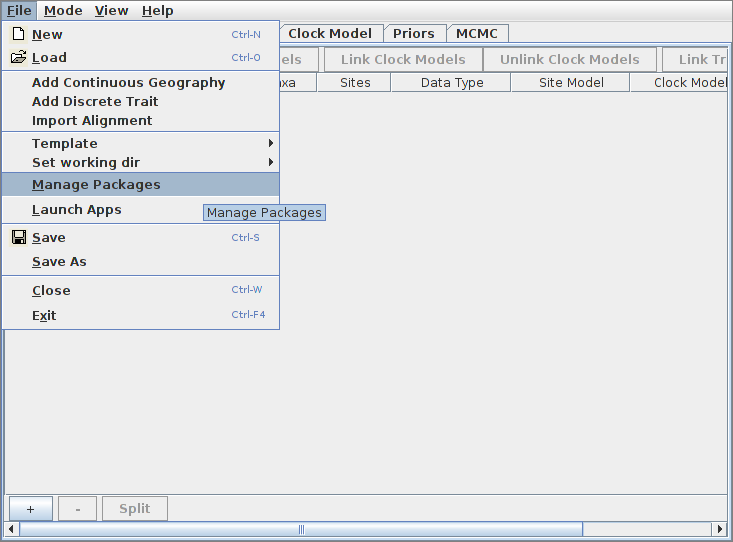
\includegraphics[width=0.800000\textwidth]{figures/beauti.png}
    \caption{}
\end{figure}

Then, ensure the ``bacter'' package is highlighted before pressing the
``Install/Upgrade'' button:

\begin{figure}
    \centering
    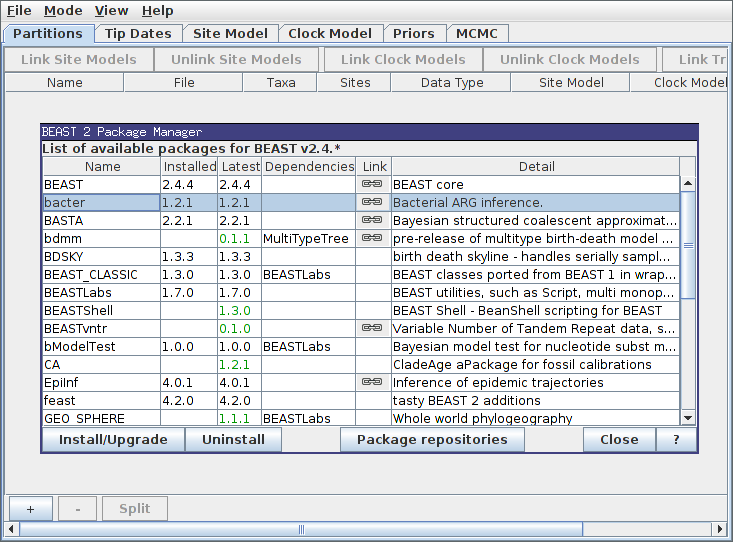
\includegraphics[width=0.800000\textwidth]{figures/package_manager.png}
    \caption{}
\end{figure}

That's it! Bacter is now installed. It is a good idea to restart BEAUti
at this point.

\section{Setting up the analysis}\label{setting-up-the-analysis}

\subsection{Choosing the Bacter BEAUti
template}\label{choosing-the-bacter-beauti-template}

Open the BEAUti program. Before doing anything else we must switch to
the Bacter template. To do this, open the file menu and from the
Template submenu select ``Bacter''.

\begin{figure}
    \centering
    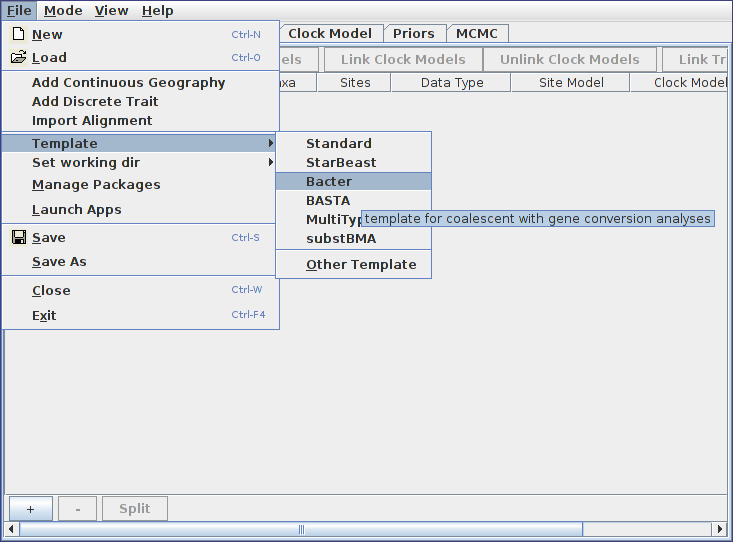
\includegraphics[width=0.800000\textwidth]{figures/template.png}
    \caption{}
\end{figure}

\subsection{Loading sequence
alignments}\label{loading-sequence-alignments}

In this tutorial we will be analyzing a subset of the E. coli data
presented in
\href{http://dx.doi.org/10.1534/genetics.116.193425}{Vaughan et al.,
Genetics, 2017}. The full data set consists of 53 individual gene
alignments, each containing 23 sequences. In order to keep our tutorial
analysis as manageable as possible, we will analyze only 12 of these
genes.

To load the alignments, select File-\textgreater{}Import Alignment and
navigate to the directory containing the tutorial data. This directory
contains 12 FASTA files, each containing the alignment for the named
gene. Since the directory contains only these files and nothing else, we
can select them all simply using Ctrl+A (or Command+A on a Mac).

\begin{figure}
    \centering
    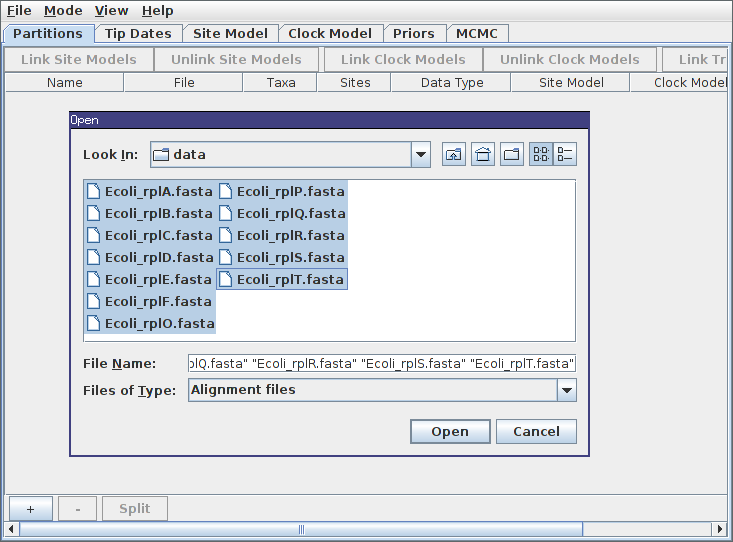
\includegraphics[width=0.800000\textwidth]{figures/load_alignments.png}
    \caption{}
\end{figure}

After pressing Open, the alignments should be visible as 12 new records
in the table. By default, each locus is assumed to have its own distinct
site, clock and ``tree'' (really ARG here) models. Since our ARGs
potentially span multiple loci, we should definitely cause the loci to
share a tree model. This is done by selecting both rows in the table by
again holding down Ctrl (or Command) and clicking each in turn.
Alternatively, you can just click on one row and then press Ctrl+A, or
Command+A on a Mac. (This is easier than clicking each row if your data
consists of many loci.) Once they're selected, press the ``Link Trees''
button on the right-hand side just above the table. In our case, we will
use shared site and clock models too, so click the ``Link Site Models''
and ``Link Clock Models'' buttons as well.

\begin{figure}
    \centering
    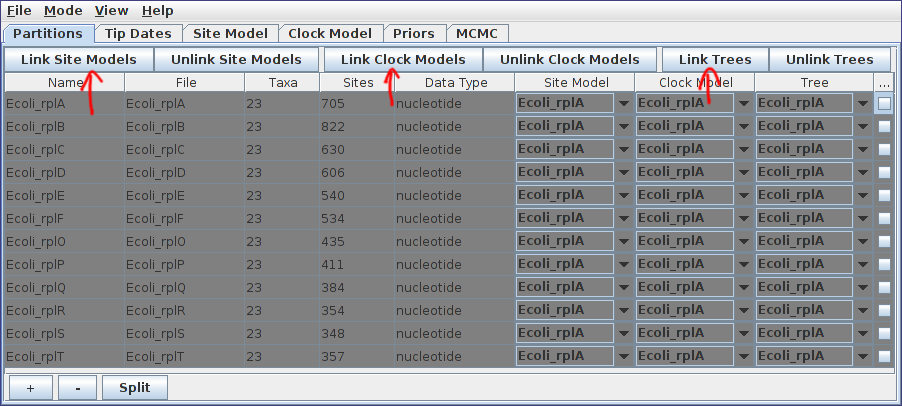
\includegraphics[width=0.800000\textwidth]{figures/link_models.png}
    \caption{}
\end{figure}

\subsection{Defining the model}\label{defining-the-model}

We will now configure the model under which the inference will be
conducted.

The data that we've loaded was sampled contemporaneously. We can
therefore ignore the Tip Dates panel. When analyzing data where the
samples were collected at very different times you'll want to include
those times in the analysis by modifying the contents of that panel.

Open the Site Model panel and set the substitution to HKY. This model is
far superior to the default Jukes-Cantor model as it allows distinct
transition/transversion rates and non-equal equilibrium base
frequencies. Leave the default initial value for kappa and the base
frequencies as ``estimated''. The site model panel should now look
similar to the following:

\begin{figure}
    \centering
    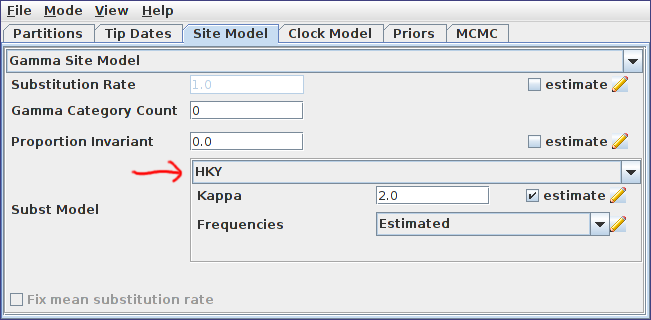
\includegraphics[width=0.800000\textwidth]{figures/site_model.png}
    \caption{}
\end{figure}

Again, because the data was sampled contemporaneously and we have no
relevant calibration information, we will ignore the Clock Model panel.
By doing this, we are implicitly deciding that time will be expressed in
expected number of substitutions per site.

Now switch to the Priors panel. See that ``Coalescent with constant
population'' is selected as the default tree prior. Expand this tree
prior by clicking on the arrow to the left of ``Tree.t''.

Uncheck the ``estimate'' checkboxes to the right of the recombination
rate (Rho) and tract length (Delta) parameters and enter the values 0.1
and 1000.0 respectively. Estimating these parameters can actually be
quite difficult, so fixing them to known values is a good idea if these
are available. In this particular case, while 1000 is a reasonable value
for the expected conversion tract length of E. Coli, fixing the
recombination rate to 0.1 is suspect. We do this solely to reduce the
computation time required for this analysis.

Select log normal priors for the population growth rate and final size
parameters, with parameters M=0 and S=2.

The priors panel should now look similar to the following:

\begin{figure}
    \centering
    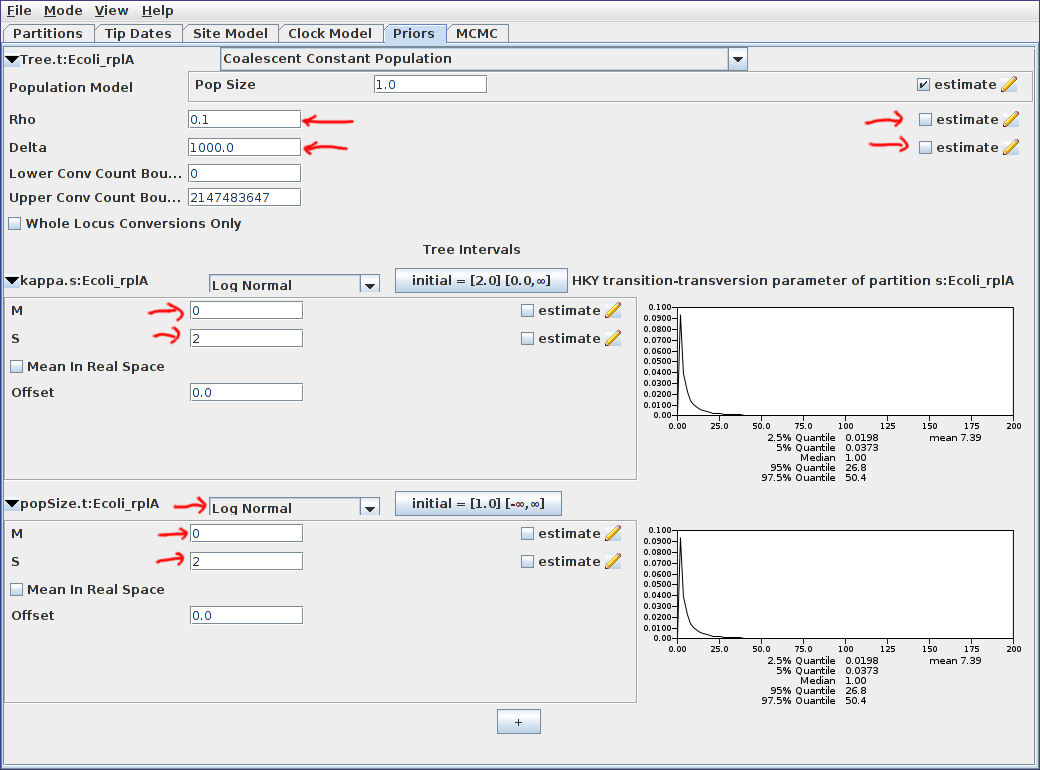
\includegraphics[width=0.800000\textwidth]{figures/priors.png}
    \caption{}
\end{figure}

Finally, switch to the MCMC panel and change the chain length to 1000000
(i.e.~10$^{6}$). This is far too short for a production run, but means
that the example analysis will complete relatively quickly. Also,
because our run is so short, we'll sample the chain of ARGs more
frequently. To do this, expand the ACGLogger.t:simulated\_data\_A
section by clicking on the arrow to the left of this line, then set the
``Log Every'' field to 1000. The MCMC panel should now look similar to
the following:

\begin{figure}
    \centering
    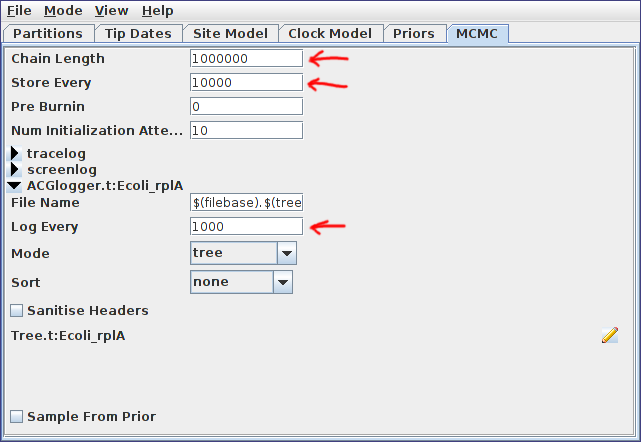
\includegraphics[width=0.800000\textwidth]{figures/mcmc_settings.png}
    \caption{}
\end{figure}

Once your analysis is set up, select File-\textgreater{}Save, navigate
to the directory you wish the analysis XML to be written to, give it a
sensible file name (for example bacter\_tutorial.xml), and press the
Save button to produce the BEAST input XML.

\textbf{Note:} If you experience difficulties using BEAUti to generate
the BEAST XML file but would like to continue immediately with the
analysis, download and use \href{xml/bacter_tutorial.xml}{this
ready-made XML file};

\section{Running the analysis}\label{running-the-analysis}

Run the analysis just as you would any other BEAST 2 analysis. That is,

\begin{enumerate}
\def\labelenumi{\arabic{enumi}.}

\item
  Start BEAST 2.
\item
  Select the XML you produced in the previous section from the file
  selection dialog box.
\end{enumerate}

Once BEAST is running, you should see output periodically printed to
standard out (if you're running BEAST from a terminal emulator) or the
output window. The analysis we've set up should take 15 minutes to
complete on a modern computer.

If you run out of time to complete the analysis, simply download the
pre-cooked \href{precooked_runs/bacter_tutorial.log}{log} and
\href{precooked_runs/bacter_tutorial.Ecoli_rplA.trees}{tree} files and
continue the tutorial using them.

\section{Analyzing the results}\label{analyzing-the-results}

During the analysis results are written to several files which can
usually located in the same directory as the directory containing the
input XML. These are:

\begin{enumerate}
\def\labelenumi{\arabic{enumi}.}

\item
  The \textbf{log} file, which ends in the extension .log and contains
  sampled parameter values,
\item
  The \textbf{tree} file, which ends in the extension .trees and
  contains sampled ARGs.
\end{enumerate}

\subsection{Parameter posteriors}\label{parameter-posteriors}

To examine the sampled parameter marginal posteriors and, more
generally, to assess the health of our analysis results, open Tracer and
load the log file. (To do this, select ``Import trace file'' from the
File menu or click the ``+'' button below and to the left of the table
in the top left corner of the Tracer window.) Shown below is the
marginal posterior for the number of conversions ancestral to our data.

\begin{figure}
    \centering
    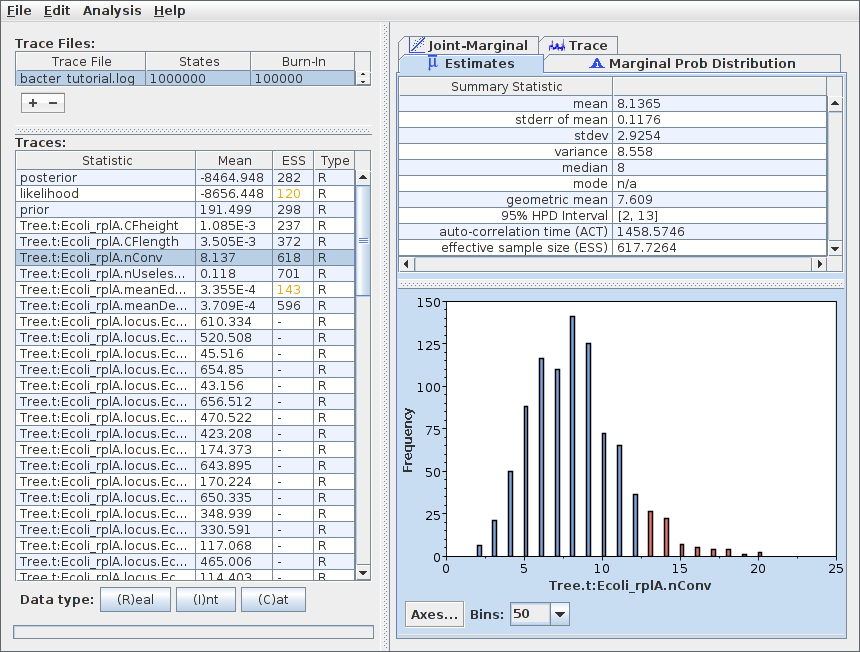
\includegraphics[width=0.800000\textwidth]{figures/tracer.png}
    \caption{}
\end{figure}

Note that the ESS for many parameters may still be extremely small after
10$^{6}$ iterations. This indicates that, as anticipated, the chain
should be run for a lot longer before the results are considered
trustworthy. We can easily continue/resume the chain just as for any
other BEAST 2 analysis, and you may wish to try this yourself. However,
in the interests of keeping the length of time needed to complete this
tutorial from becoming too long, we will now proceed to further analyse
the results we already have.

\subsection{Viewing sampled ARGs}\label{viewing-sampled-args}

The ARGs sampled during a Bacter analysis can be viewed using the
browser-based \href{http://tgvaughan.github.io/icytree}{IcyTree}
phylogenetic tree and network visualizer. Beware that the viewer
requires an up-to-date version of Firefox or Chrome to function
correctly.

To use the viewer, simply open the
\href{http://tgvaughan.github.io/icytree}{IcyTree} web page in a browser
window, select File-\textgreater{}``Load from file'', then choose the
tree file using the file chooser. Alternatively, you can simply drag the
tree file onto the IcyTree window.

Once loaded, the first ARG in the tree file is displayed. Use the comma
and period (, and .) keys to step through the file one ARG at a time or
the \textless{} and \textgreater{} keys to step in increments of 10\%.
Navigation can also be performed by clicking on the buttons in the
lower-left corner of the window with your mouse. Further information
about using IcyTree can be found by selecting items listed under the
Help menu. To generate the image below, edges were coloured by locus
(Style-\textgreater{}``Colour edges by''), the colouring legend and the
time axis were switched on (Style-\textgreater{}``Display legend'' and
Style-\textgreater{}``Display axis'').

\begin{figure}
    \centering
    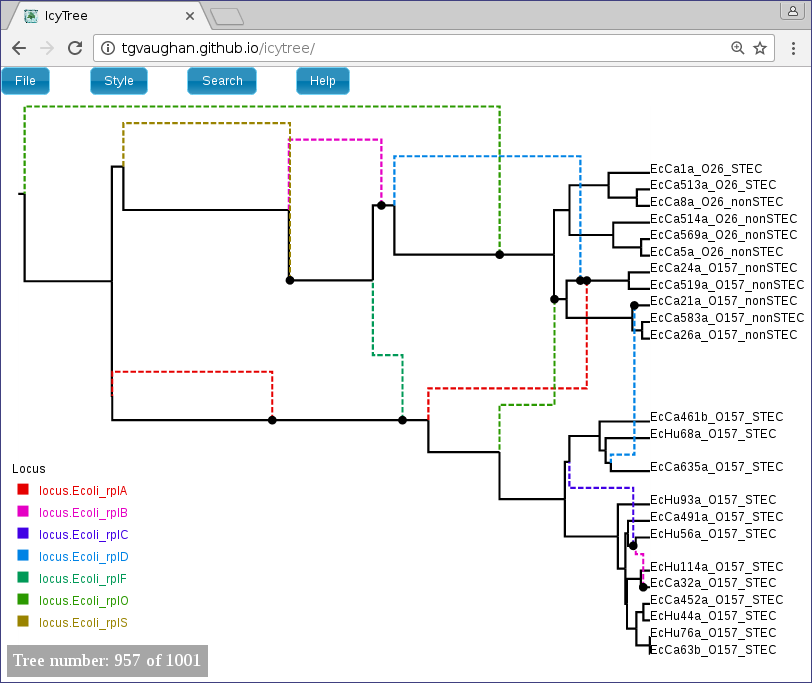
\includegraphics[width=0.800000\textwidth]{figures/icytree.png}
    \caption{}
\end{figure}

ARGs are displayed in IcyTree in a particular way. The solid lines
depict lineages belonging to the clonal frame, while dashed edges
representing the topology changes imposed on the clonal frame by
conversions. Additional information concerning a specific edge can be
viewed by hovering the mouse cursor over that edge.

It is important to remember that ARGs at the start of the file
(particularly the first) will likely be very different to the true ARG,
as this portion of the file represents ARGs sampled before convergence
of the MCMC to the true posterior. Later trees should represent
individual samples drawn from the posterior.

\subsection{Creating a summary ARG}\label{creating-a-summary-arg}

Individual ARGs sampled from the posterior are poor representations of
the inference result at best, and at worst they may be completely
misleading. This is because they contain no indication of the
uncertainty inherent in what the sequence data tells us of the events
they describe. Thus, while a single sampled ARG may contain features
that are well-supported by the data, the same ARG will likely contain
many features that have little or no support at all.

What is needed is some kind of picture of the posterior
\emph{distribution} over ARG space instead of a single point estimate.
Unfortunately, the optimal route to producing such a summary is
currently an open research question. However, Bacter provides an
implementation of an algorithm for constructing a qualitative summary
which is similar in spirit to the algorithms which BEAST and other
Bayesian phylogenetic packages use to summarize distributions over tree
space. (Refer to the
\href{http://dx.doi.org/10.1534/genetics.116.193425}{paper} for
details.)

To produce a summary ARG, open the ``AppStore'' program that is
distributed with BEAST 2. (You can also select ``Launch Apps'' from the
File menu in BEAUti.)

\begin{figure}
    \centering
    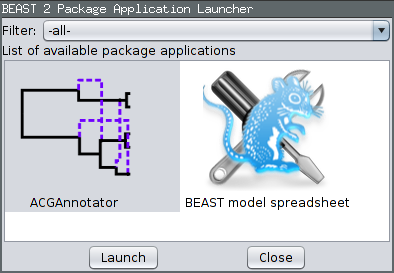
\includegraphics[width=0.800000\textwidth]{figures/appstore.png}
    \caption{}
\end{figure}

Ensure the ACGAnnotator icon is highlighted, then press the Launch
button. This will open a dialog box from which you can select the ACG
(tree) log file and the name and location of the file to which the
summary is written. In addition, you can adjust:

\begin{enumerate}
\def\labelenumi{\arabic{enumi}.}

\item
  The burn-in percentage: the percentage of the tree log file which will
  be ignored to account for the samples that were taken before the MCMC
  reached convergence.
\item
  The position summary method: this affects the way that the internal
  node ages of the summary tree are chosen. The default is to use the
  mean of the node ages present in the sampled ARGs.
\item
  The posterior conversion support threshold: this is the percentage of
  sampled ARGs which must contain a given conversion for it to be
  included in the summary tree. (This is conceptually similar to the
  threshold for clade inclusion in a majority-rule consensus tree.)
\end{enumerate}

For this tutorial, ensure the ACG (tree) log file generated by the above
analysis is selected and choose summary.tree as the output file name.
Leave the burn-in fraction at 10\% and keep MEAN as the position summary
method, but lower the conversion support threshold to 20\%. This means
that conversions will only have to appear in 20\% of the sampled ARGs to
be included in the summary. The dialog box should now look like the
following image:

\begin{figure}
    \centering
    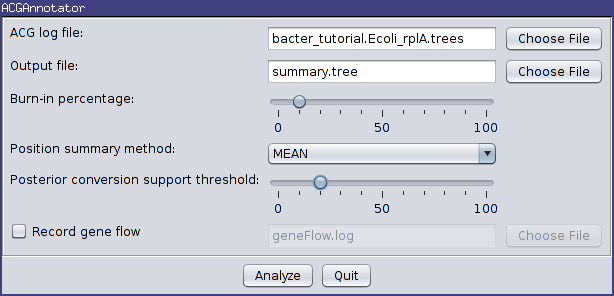
\includegraphics[width=0.800000\textwidth]{figures/acgannotator.png}
    \caption{}
\end{figure}

Pressing the ``Analyze'' button will bring up an additional window which
will report on the progress of creating the summary tree. As there are
only a few hundred ARGs present in our log file, this process should
only take a few seconds. Once it is complete, press the Close button.
You can also exit the AppStore.

Loading the file summary.tree in IcyTree should produce something
similar to the following figure. (Edges have been coloured by ``locus'',
and labelled with their posterior support. Error bars indicating the
95\% HPD intervals for the age of each ancestral event have also been
included.)

\begin{figure}
    \centering
    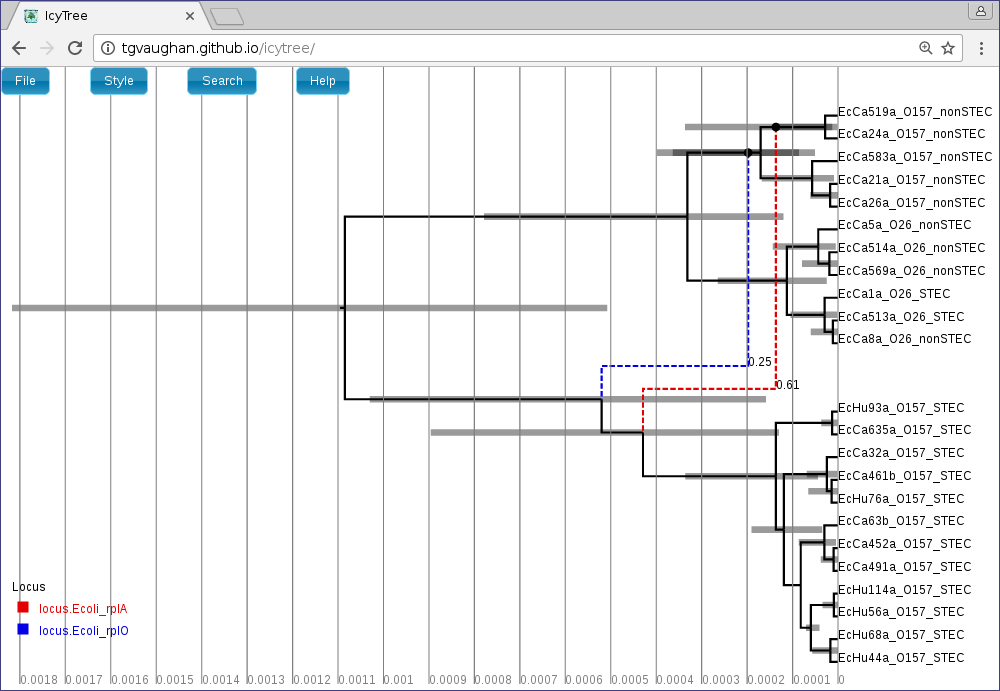
\includegraphics[width=0.800000\textwidth]{figures/summary.png}
    \caption{}
\end{figure}

This summary suggests that our E. coli dataset only has evidence for one
or two conversions: one on the rplA gene with \textasciitilde{}60\%
support and one on the rplO gene with much lower support. Note however,
that this summary does not at all rule out the possibility of many other
conversion events ancestral to the data: it simply indicates that only
these conversions occur in roughly the same place in at least 20\% of
the posterior samples.

This distinction is backed up by the marginal posterior distribution for
the number of conversion events in the graph shown in the tracer figure
above, which has a median of 8 events - still very small, but four times
the number appearing in the summary. The discrepancy is likely made up
of conversions that produced very little or no signal in the data.

\section{Wrapping up}\label{wrapping-up}

This completes our introductory Bacter tutorial. There are other
features that are not covered here, such as the ability to perform
inference under different parametric and non-parametric models of
population dynamics. Tutorials explaining these features will appear in
the near future on the \href{https://tgvaughan.github.io/bacter}{Bacter
web page}.

\section{Useful Links}\label{useful-links}

\begin{itemize}

\item
  Bacter website and documentation:
  \url{https://tgvaughan.github.io/bacter}
\item
  BEAST 2 website and documentation: \url{http://www.beast2.org/}
\item
  Join the BEAST user discussion:
  \url{http://groups.google.com/group/beast-users}
\end{itemize}

%%%%%%%%%%%%%%%%%%%%%%%
% Tutorial disclaimer %
%%%%%%%%%%%%%%%%%%%%%%%
% Please do not change the license
% Add the author names and relevant links
% Add any other aknowledgments here
\href{http://creativecommons.org/licenses/by/4.0/}{
\includegraphics[scale=0.8]{figures/ccby.pdf}} This tutorial was written by Tim Vaughan for \href{https://taming-the-beast.github.io}{Taming the BEAST} and is licensed under a \href{http://creativecommons.org/licenses/by/4.0/}{Creative Commons Attribution 4.0 International License}. 


%%%%%%%%%%%%%%%%%%%%
% Do NOT edit this %
%%%%%%%%%%%%%%%%%%%%
Version dated: \today



\newpage

%%%%%%%%%%%%%%%%
%  REFERENCES  %
%%%%%%%%%%%%%%%%

\printbibliography[heading=relevref]


\end{document}